\documentclass{book}
\usepackage{graphicx} % new way of doing eps files
\usepackage{rotating} % for sideways
\usepackage{multirow} % for \multirow
\usepackage{url}      % for \url
\usepackage{hyperref} % for \href
\usepackage{listings} % nice code layout
\usepackage[usenames]{color} % color
\definecolor{listinggray}{gray}{0.9}
\definecolor{graphgray}{gray}{0.7}
\definecolor{ans}{rgb}{1,0,0}
\definecolor{blue}{rgb}{0,0,1}
% \Code{title}{label}{file}{language}
\newcommand{\Code}[4]{
  \lstset{language={#4}}
  \lstset{backgroundcolor=\color{listinggray},rulecolor=\color{blue}}
  \lstset{linewidth=\textwidth}
  \lstset{commentstyle=\textit, stringstyle=\upshape,showspaces=false}
  \lstset{frame=tb}
  \lstinputlisting[caption={#1},label={#2}]{#3}
}

% source: http://stackoverflow.com/questions/741985/latex-source-code-listing-like-in-professional-books
% \SourceCode{language}{caption}{label}{file_path}
\newcommand{\SourceCode}[4]{
  % #1 = language, usually first letter is in upper case
  % #2 = caption
  % #3 = label
  % #4 = path
  \lstset{language=#1}
  \lstset{
    commentstyle=\color{orange}\textit,
    basicstyle=\footnotesize\ttfamily, % Standardschrift
    % numbers=left,               % Ort der Zeilennummern
    numberstyle=\tiny,          % Stil der Zeilennummern
    % stepnumber=2,               % Abstand zwischen den Zeilennummern
    numbersep=5pt,              % Abstand der Nummern zum Text
    tabsize=2,                  % Groesse von Tabs
    extendedchars=true,         %
    breaklines=true,            % Zeilen werden Umgebrochen
    keywordstyle=\color{red},
    frame=b,
    % keywordstyle=[1]\textbf,    % Stil der Keywords
    % keywordstyle=[2]\textbf,    %
    % keywordstyle=[3]\textbf,    %
    % keywordstyle=[4]\textbf,   \sqrt{\sqrt{}} %
    stringstyle=\color{blue}\ttfamily, % Farbe der String
    showspaces=false,           % Leerzeichen anzeigen ?
    showtabs=false,             % Tabs anzeigen ?
    xleftmargin=17pt,
    framexleftmargin=17pt,
    framexrightmargin=5pt,
    framexbottommargin=4pt,
    backgroundcolor=\color{listinggray},
    % backgroundcolor=\color{lightgray},
    showstringspaces=false      % Leerzeichen in Strings anzeigen ?
  }
  \lstinputlisting[caption={#2},label={#3}]{#4}
}

\usepackage{floatflt}
%\usepackage{cscilabs}

\newcounter{examplecounter}
\newenvironment{example}{\begin{quote}%
    \refstepcounter{examplecounter}%
  \textbf{Example \arabic{examplecounter}:}%
  \quad
}{%
\end{quote}%
}

\topmargin 0in
\textheight 8.5in
\textwidth 6.5in
\evensidemargin 0in
\oddsidemargin 0in

\renewcommand{\chaptername}{Lab}


\title{
{\Huge Baylor University} \\
\vspace{1in}
{\large Department of} \\
{\Large Electrical and Computer Engineering}\\
\vspace{1in}
{\Large ELC 5311 (graduates), 4396(undergrad)} \\
{\Huge Advanced Digital Logic Laboratories} \\
}
\author{
Keith Schubert\\
Professor\\
Department of Electrical and Computer Engineering\\
Baylor University
}
\date{}

\makeindex

\begin{document}

\baselineskip=1.05\normalbaselineskip

\maketitle

\tableofcontents

%\listoffigures

%\listoftables

\pagenumbering{arabic}

\chapter{Nexys 4 DDR Programming}

\section{Project Setup}

\begin{tabular}{l@{:}c}
Family & Artix-7\\
Sub-Family & a1000t\\
Package & csg324\\
Speed Grade & -1\\
\end{tabular}

Select ``xc7a100tcsg324-1''



\section{Passthrough}

We are going to begin with a simple project to turn on LEDs when the switch under them is on.  There are eight switches (called sw$\langle 7\rangle$ \ldots sw$\langle 0\rangle$), and eight LEDs  (called Led$\langle 7\rangle$ \ldots Led$\langle 0\rangle$).  Our first easy part will be to assign the LEDs to be identical to the switches, see Code~\ref{code:passthroughsimple}.

\Code{Verilog code for pass-through}{code:passthroughsimple}{../labs/lab_01/pass_through_simple.v}{Verilog}

This code simply passes the switches through to the LEDs, but it demonstrates the \textbf{assign} statement, which is one of our basic ways of designing combinational circuits.  The other important thing is to have a Xlilinx Design Constraints file (XDC) file.  Note before vivado (Xilinx products before version 7 of their FPGAs, i.e. Spartan-6 and below) they used a different file type called a user constraints file (UCF).  The big difference is in how timing is handled, which we will get into later in the course, for now I just want you to be aware that there are two standards and XDC should be used on FPGA families with a 7 or later.  The book will use a UCF because it is working on a Spartan-3 board.  An example of an XDC file is below.

\Code{Xlilinx Design Constraints file (XDC)}{code:XDCpassthroughsimple}{../code/common/Nexys4DDR_Master.xdc}{tcl}

\section{Making a Counter for the Seven Segment Display}

Now we want to drive the seven segment display.  All the cathodes of the LEDs in the same position are hooked together.  So for example, all four of the top LEDs' cathodes are hooked together, as are all the cathodes of the upper right, and so on.  The top LED is called A or seg$\langle 0\rangle$, the letters and numbers proceed clockwise, and the middle segment is G or seg$\langle 6\rangle$.  Each digit also has a decimal point, which is called dp, and their cathodes are also connected.   The FPGA does sink the current in this case (\emph{Why can it sink what it couldn't source?}), so a zero turns the LED on if the anode was also sourced.

To drive the seven segment display we will then need to convert from a 4 bit binary number to the seven segment display cathode pattern.  We will leave the decimal point off.  This can be seen in Code~\ref{code:sseg}.

\Code{Verilog code for converting 4 bit binary to sseg.}{code:sseg}{../labs/lab_01/sseg_driver.v}{verilog}

All the anodes for a digit are hooked together, so since there are four digits there are four anode lines (called an$\langle 3\rangle$ \ldots an$\langle 0\rangle$).  The output of the fpga is not strong enough to supply all the current for the LEDs, so a pnp transistor is used to switch power (\emph{Why does a pnp switch power better, and an npn switch ground better?}).  This means a zero, is needed to turn the pnp on and a 1 will turn it off.

This slicing allows control of 32 LEDs with 12 wires and one fourth can be on simultaneously.  Since each LED will be off three fourths of the time, we need to switch them faster than the eye can see, and since the diode's pn junction holds charge for a bit (discharges like a capacitor, why?) and thus continues to glow, and the eye continues to see light for a bit.  The Nexys 4 board has a 100MHz clock, so we need to count to about 2 million, which is 21 bits.  We thus need a counter that can count to whatever number of bits we want.

\Code{Verilog code for counting a parameterized number of bits.}{code:count}{../labs/lab_01/counter.v}{verilog}

To show this off, we will have a slow count displaying, with say a count around a second or so.  This is about 50, which is close enough to 6 bits for our use.  We will thus first make a 27 bit counter, triggering the rotation of the anodes off bits 18 and 19, and the next count off bit 26.  We will thus make one more counter, this time with 32 bits so we can drive all 8 segments.  We just need to change our top level module and xdc to reflect this.



\chapter{Barrel Shifter}

Do Experiment 3.11.1 Multifunction Barrel Shifter from the book.

\chapter{Adders and Complexity}

\section{Introduction}

Addition is a fundamental part of any ALU and can be easily produced in Verilog by just using ``$+$''.  You will get an adder that is inferred for your FPGA.  The actual adder varies wildly from simple ripple adders, to specialized pre-built hardware blocks.  We are going to explicitly build three different adders with very different complexities and compare them.

\subsection{Ripple Adders}

This is the technique that is covered in digital logic.  Basically, full bit adders, see Figure~\ref{f-half_full_add}, are created and cascaded together.  The carry bit from the previous full adder must arrive before the result is added.  The resulting valid carries thus ripple down to the most significant bit (hence the name).  Adding $n$ bit numbers, thus takes the propagation time of $n+1$ levels of logic, i.e. it is O(n) in time to calculate addition.  Thus if 32 bit numbers are added on fast logic (1ns per stage/gate) the process would take 33ns.  This is way too slow.  On the bright side, none of the gates take more than 2 inputs so the size of the gates is O(1).

\begin{figure}
\caption{(left) Half Adder, (right) Full Adder}\label{f-half_full_add}
\begin{center}
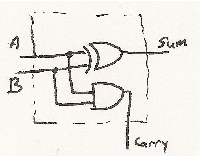
\includegraphics{ha.png} \hspace{.2in} 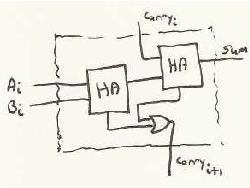
\includegraphics{fa.png}
\end{center}
\end{figure}

\subsection{Conditional Sum}
Conditional sum is a divide and conquer algorithm, and hence exploits binary tree parallelism.  The algorithm works by calculating both possible results for each bit (if carry in was 1 or 0), then performing paired conditional concatenation using the actual carry bit of the lower number, see Figure~\ref{f-cond_sum_add}.

\begin{figure}
\caption{Conditional Sum Adder (above), and its sub-blocks (below, left and right).}\label{f-cond_sum_add}
\begin{center}
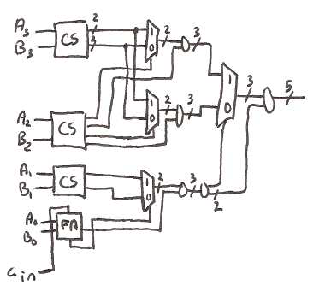
\includegraphics{conditional_sum.png}\\\vspace{.2in}
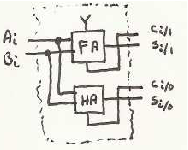
\includegraphics{cs_4out.png} \hspace{.2in} 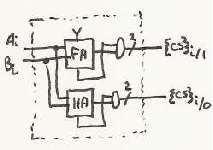
\includegraphics{cs_2out.png}
\end{center}
\end{figure}

\begin{enumerate}
    \item form conditional terms for each digit in summation $\rightarrow$ (digit with carry, digit without carry) = ($x_i+y_i+1$,$x_i+y_i$)
    \item group by twos from right and for both conditional values in the right parenthesis form the result as follows:
    \begin{enumerate}
        \item the leftmost bit of the two terms on the right are the carry bits used to select the term on the left
        \item concatenate the appropriate term on the left (picked by carry) with each term on right after removing the parity bits of the right terms
    \end{enumerate}
    \item continue pairings until only 1 term remains. pick right number if $c_{in}=0$ else pick left.
\end{enumerate}

\begin{example}
 Add $x=0110$ and $y=1111$ by conditional sum and indicate if overflow occurred.

        {\color{ans}
        \begin{tabular}{cccc}
          0+1 & 1+1 & 1+1 & 0+1 \\
          $\downarrow$ & $\downarrow$ & $\downarrow$ & $\downarrow$ \\
          (10,01) & (11,10) & (11,10) & (10,01) \\
          $\searrow$ & $\swarrow$ & $\searrow$ & $\swarrow$ \\
          \multicolumn{2}{r}{(101,100} & \multicolumn{2}{l}{(110,101)} \\
          \multicolumn{2}{c}{$\searrow$} & \multicolumn{2}{c}{$\swarrow$} \\
          \multicolumn{4}{c}{(10110,10101)} \\
          \multicolumn{4}{c}{1 0101} \\
        \end{tabular}

        No overflow occurred (added a positive and negative number).
        }
\end{example}



\begin{example}
    Calculate $7-8$ by conditional sum.

    {\color{ans}

    $7=0111$ and $-8=1000$

    \begin{tabular}{cccc}
    $\;$ 0       & 1          & 1          & 1          \\
      +1         & 0          & 0          & 0          \\ \hline
      (10,01)    & (10,01)    & (10,01)    & (10,01)    \\
      $\searrow$ & $\swarrow$ & $\searrow$ & $\swarrow$ \\
      \multicolumn{2}{c}{(100,011)} & \multicolumn{2}{c}{(100,011)} \\
      \multicolumn{2}{c}{$\quad\searrow$} & \multicolumn{2}{c}{$\swarrow\quad$} \\
      \multicolumn{4}{c}{(10000,01111)} \\
    \end{tabular}

    Since this was done as addition no carry-in was set so the solution is \begin{tabular}{r|l} 0 & 1111 \\ \hline \end{tabular} or $-1$ in signed base ten.

    }
\end{example}


\begin{example}
Add by conditional sum $x=01100110$ and $y=00110011$.

{\color{ans}
\noindent
\begin{tabular}{rrrrrrrr}
$0+0$ & $1+0$ & $1+1$ & $0+1$ & $0+0$ & $1+0$ & $1+1$ & $0+1$ \\
$\downarrow$ & $\downarrow$ & $\downarrow$ & $\downarrow$ & $\downarrow$ & $\downarrow$ & $\downarrow$ & $\downarrow$ \\
$(01,00)$ & $(10,01)$ & $(11,10)$ & $(10,01)$ & $(01,00)$ & $(10,01)$ & $(11,10)$ & $(10,01)$ \\
$\searrow$ & $\downarrow$ & $\searrow$ & $\downarrow$ & $\searrow$ & $\downarrow$ & $\searrow$ & $\downarrow$ \\
\multicolumn{2}{r}{$(010,001)$} & \multicolumn{2}{r}{$(110,101)$} & \multicolumn{2}{r}{$(010,001)$} & \multicolumn{2}{r}{$(110,101)$} \\
& $\searrow$ & & $\swarrow$ & & $\searrow$ & & $\swarrow$  \\
&  & \multicolumn{2}{c}{$(01010,01001)$} &  &  & \multicolumn{2}{c}{$(01010,01001)$ }  \\
&  &  & $\searrow$ &  & $\swarrow$ &  &  \\
&  &  & \multicolumn{3}{c}{$(010011010,010011001)$} &  &  \\
&  &  & \multicolumn{3}{c}{$0 \, 10011001$} &  &  \\
\end{tabular}
}
\end{example}

Why go through this?  First, by a folk theorem of Dr. Alan Laub, ``\emph{What is hard for us tends to be easy for computers (and vice versa)}.''  In reality this process is really easy for a computer to do.  Second, the process is highly parallel, so it can be done very fast.  If the numbers to be added are n bits long this takes $2(\log_2(n)+1)$ levels of logic, much better than the $n+1$ levels of logic required by ripple calculations.  Thus it is O(log(n)) in time complexity.  For example, for adding the 32 bit numbers considered already, conditional sum would take $2(\log_2(32)+1)=12$ levels of logic, so on the fast logic described it would be 12ns, a huge improvement.

\subsection{Carry-Lookahead}

This is also referred to as lookahead carry.  Assume $x+y=z$.  Pre-generate all carries with 2-level logic. Usually form (g,p,c) generate, propagate, carry.
\begin{eqnarray}
G_i & = & x_i \cdot y_i \\
P_i & = & x_i + y_i \\
C_i & = & G_i + P_i \cdot C_{i-1} \\
    & = & G_i + P_i \cdot (G_{i-1} + P_{i-1} \cdot C_{i-2}) \\
    & = & G_i + P_i \cdot G_{i-1} + P_i \cdot P_{i-1} \cdot C_{i-2} \\
    & = & G_i + P_i \cdot G_{i-1} + P_i \cdot P_{i-1} \cdot G_{i-2} +
    \ldots + P_i \cdot P_{i-1} \cdot \ldots \cdot P_0 \cdot C_{in}
\end{eqnarray}

This method is very fast (regardless of size it take 5 levels of logic) but requires large gates for problems of reasonable size (even 16 or 32 bit numbers) and thus has problems with fan-in, fan-out, and size.

Often blocks of a number are handled with lookahead, and the blocks are connected in some fashion (for example ripple) to get the net result (i.e. just like single bit adds from a full adder are connected to propagate the carry bit, blocks or 4, 8, or more could be handled lookahead then connected to propagate the carry bit between them to handle a larger number, say 32 bits).  Even better than cascading (ripple connection) the adders, is to us group carry-lookahead, in which each of the carry-lookahead adders output their group propagate and group generate variables to a circuit that generates the carry-in bits for each group.  It takes 5 logic levels to generate the carries to each individual carry-lookahead adder, and each adder then takes 5 levels of logic to get the result, for a total of 10 levels of logic.  For the example of adding 32 bit numbers with fast logic, it would take 10ns with group carry-lookahead adders (probably four or eight bits in a group).


\begin{example}
Specify the equations of a two bit binary adder with carry in (i.e.: one equation for each of the sum bits and one equation for the carry out).  Put the equations in sum of products form.

{\color{ans}Sol:
Let the two numbers to be added be $A_1 A_0$ and $B_1 B_0$.  Let the resulting sum be $S_1 S_0$.  Let the carries be $C_{in}$ and $C_{out}$.  Finally, let $C_0$ be the carry from the first bit added (saves writing).
\begin{eqnarray}
S_0 & = & A_0 \oplus B_0 \oplus C_{in} \\
C_0 & = & A_0\cdot B_0 + A_0\cdot C_{in} + B_0\cdot C_{in} \\
S_1 & = & A_1 \oplus B_1 \oplus C_0\\
C_{out} & = & A_1 \cdot B_1 + A_1 \cdot C_0 + B_1 \cdot C_0
\end{eqnarray}
Putting this in sum of products form yields
\begin{eqnarray}
S_0 & = & A_0' \cdot B_0' \cdot C_{in} +
          A_0' \cdot B_0 \cdot C_{in}' +
          A_0 \cdot B_0' \cdot C_{in}' +
          A_0 \cdot B_0 \cdot C_{in} \\
S_1 & = & A_1' \cdot B_1' \cdot (A_0\cdot B_0 + A_0\cdot C_{in} + B_0\cdot C_{in}) +
          A_1' \cdot B_1 \cdot (A_0\cdot B_0 + A_0\cdot C_{in} + B_0\cdot C_{in})' + \\
    & & \qquad A_1 \cdot B_1' \cdot (A_0\cdot B_0 + A_0\cdot C_{in} + B_0\cdot C_{in})' +
          A_1 \cdot B_1 \cdot (A_0\cdot B_0 + A_0\cdot C_{in} + B_0\cdot C_{in}) \\
    & = & A_1' \cdot B_1' \cdot A_0\cdot B_0 + A_1' \cdot B_1' \cdot A_0 \cdot C_{in}
          + A_1' \cdot B_1' \cdot B_0\cdot C_{in} \\
    & & \qquad
          + A_1' \cdot B_1 \cdot (A_0'\cdot B_0' + A_0'\cdot C_{in}' + B_0'\cdot C_{in}') \\
    & & \qquad
          + A_1 \cdot B_1' \cdot (A_0'\cdot B_0' + A_0'\cdot C_{in}' + B_0'\cdot C_{in}') \\
    & & \qquad
          + A_1 \cdot B_1 \cdot A_0\cdot B_0 + A_1 \cdot B_1 \cdot A_0\cdot C_{in}
           + A_1 \cdot B_1 \cdot B_0\cdot C_{in} \\
    & = & A_1' \cdot B_1' \cdot A_0\cdot B_0 + A_1' \cdot B_1' \cdot A_0 \cdot C_{in}
          + A_1' \cdot B_1' \cdot B_0\cdot C_{in} \\
    & & \qquad
          + A_1' \cdot B_1 \cdot A_0'\cdot B_0' + A_1' \cdot B_1 \cdot A_0'\cdot C_{in}'
          + A_1' \cdot B_1 \cdot B_0'\cdot C_{in}' \\
    & & \qquad
          + A_1 \cdot B_1' \cdot A_0'\cdot B_0' + A_1 \cdot B_1' \cdot A_0'\cdot C_{in}'
          + A_1 \cdot B_1' \cdot B_0'\cdot C_{in}' \\
    & & \qquad
          + A_1 \cdot B_1 \cdot A_0\cdot B_0 + A_1 \cdot B_1 \cdot A_0\cdot C_{in}
           + A_1 \cdot B_1 \cdot B_0\cdot C_{in} \\
C_{out} & = & A_1 \cdot B_1 + A_1 \cdot (A_0\cdot B_0 + A_0\cdot C_{in} + B_0\cdot C_{in}) \\
   & & \qquad + B_1 \cdot (A_0\cdot B_0 + A_0\cdot C_{in} + B_0\cdot C_{in}) \\
    & = & A_1 \cdot B_1 + A_1 \cdot A_0\cdot B_0 + A_1 \cdot A_0\cdot C_{in} + A_1 \cdot B_0\cdot C_{in} \\
   & & \qquad + B_1 \cdot A_0\cdot B_0 + B_1 \cdot A_0\cdot C_{in} + B_1 \cdot B_0\cdot C_{in}
\end{eqnarray}
}
\end{example}

\section{Generate}

The Verilog generate command is a powerful tool.  Consider the code to generate a ripple carry adder below.
\Code{Ripple adder}{ra}{../code/adder/ripple.v}{verilog}



\section{Assignment}

Build 8-bit adders for:
\begin{enumerate}
\item ripple carry adder
\item conditional sum adder
\item block carry lookahead, with 4-bit blocks
\end{enumerate}

\chapter{PWM Dimmer}

\section{Pulse Width Modulation}

Pulse width modulation is a direct way to drive analog devices with a digital output.  Since it does not require any additional equipment, it is very popular in a number of applications.  The basic idea is similar to a bang-bang control\footnote{Bang-bang controls are best known in thermostats, where the system is on or off, but not in any state in between.}, but unlike typical bang-bang controls the cycle time is set very short so the output is effectively a weighted averaged, since most systems function like a low pass filter.  The weighting is due to the duty cycle, which is the fraction of the cycle time that the output is on/high.  If the output power of the digital line is $P$ and the duty cycle is $d$, then the effective power is $P_e=d P$.

Pulse width modulation is very effective in simple servos, LEDs, and other simple devices that need to be driven by a digital controller.  They are particularly common in hobby applications, but also find use in telecommunications, monitors, fans, and pumps.  You can time them off the leading edge, trailing edge, or center of the edges, which results in three slightly different versions, but all are identified as PWM versions.

\section{Assignment for all}

Do Experiment 4.7.2 PWM and LED Dimmer from the Book.

\section{Graduate Student Additional Work}

Incorporate your dimmer in the LED time-multiplexing circuit of 4.5.1.  In order to do this, you need more than 8 switches.  Since this is only for testing, use switches 0-7 for the original circuit and also use 0-3 for the dimmer.  This has duplication but does not produce any issues for demonstration purposes.  Note: basic code for the system is available in the starter code from the book available from the class GitHub. 

\chapter{Parking Lot}

\section{Is the Lot Full}

Knowing if a parking lot is full, allows us to advise motorists as well as store usage data to plan for future additions.  Since many parking lots were not designed around controlling entrance and exit of vehicles or people, retrofitting a parking lot for a counter becomes an issue.  Additionally, many entrances are two-way, creating further complications.  You are part of a team that will be building a sensor for retrofitting small parking lots ($<100$ cars).  As such the expense of cutting through the road to put car sensors is prohibitive, so a light based sensor (see Figure 5.11 in the book) has been selected.  In 5.5.3, the method of determining if a car is entering or exiting is outlined, but there are many other exceptions, such as a car starting to enter and then backing up.  You may assume the sensors are spaced to be able to identify a car from smaller objects like people or bikes since the latter will only trip one sensor at a time, while cars will trip both.  Such a system could be tricked by two people, however, so you may assume for simplicity that the lanes to the parking lot are not high foot traffic areas.

\section{Task}

Design, implement, test, and document your solution to 5.5.3 in the textbook.  For graduate students: assume there are two entry/exit points so your counter must handle multiple sensor units sending inc and dec signals. 

\chapter{Babbage Difference Engine Emulation Circuit}

\section{Newton's Differences}
Newton's method of differences is foundational to interpolation, where it comes in as divided differences, and as a simplification of calculus.  Essential each difference is approximating a derivative.  You calculate the differences between successive steps, say $f(n)$ and $f(n-1)$ for the values of $n$ that are in a region of interest.  If the differences are constant you are done, if not take the differences of these.  Repeat until they become constant.  Since differences approximate derivatives, repeatedly performing differences on finite polynomials will eventually result in a constant.  For example consider performing Newton's differences on $f(n)=n^2$,

\noindent
\begin{tabular}{c|ccccc}
$n$                                                 & 0 & 1 & 2 & 3 & 4  \\\hline
$f(n)=n^2$                                          & 0 & 1 & 4 & 9 & 16 \\
$f_1=f(n)-f(n-1)=n^2-(n-1)^2=n^2-(n^2-2n+1)=2n-1$   & - & 1 & 3 & 5 & 7  \\
$f_2=f_1(n)-f_1(n-1)=2n-1-(2(n-1)-1)=2n-1-(2n-3)=2$ & - & - & 2 & 2 & 2  \\
\end{tabular}

Notice after two differences you end up with a constant difference of $2$, which is the same as the second derivative of the function.  Note this is not an accident, since it is following the leading coefficient.  It works for both the points and algebraically due to the leading coefficent being the important part, but note the intermediate terms are not exactly the derivative\footnote{This leads to the need for Newton to develop infinitesimals to fix it, that in turn led to Calculus}, but are needed to keep the scales right given the jump between each integer.  

You can also try this on $f(n)=n^3$ (or any other finite polynomial),

\noindent
\begin{tabular}{c|ccccc}
$n$                                                      & 0 & 1 & 2 &  3 &  4  \\\hline
$f(n)=n^3$                                               & 0 & 1 & 8 & 27 & 64 \\
$f_1=f(n)-f(n-1)=n^3-(n-1)^3=3n^2-3n+1$                  & - & 1 & 7 & 19 & 37  \\
$f_2=f_1(n)-f_1(n-1)=3n^2-3n+1-(3(n-1)^2-3(n-1)+1)=6n-6$ & - & - & 6 & 12 & 18  \\
$f_3=f_2(n)-f_2(n-1)=(6n-6)-(6(n-1)-6)=6$                & - & - & - &  6 &  6  \\
\end{tabular} 

For non-polynomials or infinite polynomials it will keep going but the intermediates are meaningful due to Taylor Series approximation.  If you are interested in going further with this take a course on numerics (a much beloved field of mine...), though this is as much as we need.  

\section{Babbage's Difference Engine}
This is what Babbage implemented in his famous difference engine (and expanded on in the analytic engine), and which Lady Ada Lovelace became the first programmer due to her love of and skill with mathematics.  Together this idea brings together three of the great events of computer history, which is why we will build it (something Babbage was not able to due to the cost and time.   The process is nicely described in Experiment 6.5.7 Babbage Difference Engine Emulation Circuit from the book.  Steps 1-4 are the methodology, step 5 just asks you to redo the design for a second system.  Design and implement for both polynomials ($f(n)=2n^2+3n+5$ and $h(n)=n^3+2n^2+2n+1$).  Calculate the algebraic form

\section{Graduate Students}
Babbage's difference engine can be generalized to where you can input the parameters for each of the sub-functions.  Design a system that would work for any second or third order polynomial by inputting coefficients.  Include the design with explanation (you don't have to build it) in your report in addition to the work the undergrads must do.
 



\appendix

\chapter{Github}

Git is a version control system originally developed by Linus Torvalds to do the Linux OS development.  Github is a git web service that I will be using to develop the labs.  You can get the manual and code from:

\url{https://github.com/KeithEvanSchubert/Advanced_Digital_Logic.git}



\end{document}
